\section{Introduction of 7 Mental Disorders}
\label{apd:dis_intro}
Here, we briefly introduce 7 mental disorders studied in our paper, listing their typical symptoms in Table \ref{tab:disease_intro} for better understanding of these mental disorders.

\begin{table}[h]
    \small
    \centering
    \begin{tabular}{m{2.2cm}|m{4cm}}
    \hline
    Disease          & Typical Symptoms \\
    \hline
    ADHD             & inattention; hyperactivity and impulsivity.         \\
    \hline
    Anxiety          &  excessive fear and worry; panic attacks; anxious mood.       \\
    \hline
    Bipolar Disorder & drastic shift in mood and energy; experience periods of mania and depression.        \\
    \hline
    Depression       &  depressed mood; loss of pleasure or interest; poor concentration; guilty feelings; suicidal ideas.      \\
    \hline
    Eating Disorder  &  intense fear of gaining weight; binge and purge; rumination.         \\
    \hline
    OCD              & obsession; compulsion.         \\
    \hline
    PTSD             &  often develops after a shocking, dangerous event; flashbacks; bad dreams.        \\
    \hline
    \end{tabular}
    \caption{7 mental disorders detected in our work with their typical symptoms.}
    \label{tab:disease_intro}
\end{table}


\section{Detailed Data Statistics}
\label{apd:stats}

For the disease detection dataset (\S \ref{sec:mdd_dataset}), we show the number of users suffering from each disease in Table \ref{tab:disease_detect_count}. The distribution of the 7 diseases are similar to SMHD \citep{cohan2018smhd}, and the  training/validation/testing set is 8:1:1. Specifically, the MDD dataset in \citet{Zhang2022SymptomIF} contains 9 mental disorders, and we removed the labels of \textit{Schizophrenia} and \textit{Autism} which cannot be handled by the symptom identification model (\S \ref{sec:symp_screen}).
% 由于症状识别模型只包括7种疾病,所以我们在这里去掉了数据集中这7种疾病之外的两种疾病的标签。
\begin{table}[h]
    \small
    \centering
    \begin{tabular}{lc}
    \hline
    Disease          & \# Users \\
    \hline
    Depression       & 3105         \\
    Anxiety          & 2239         \\
    % Autism           & 716         \\
    ADHD             & 2374         \\
    Bipolar Disorder & 1366         \\
    OCD              & 753          \\
    PTSD             & 391          \\
    % Schizophrenia    & 345          \\
    Eating Disorder  & 138          \\
    \hline
    \end{tabular}
    \caption{Number of users suffering from each disease in the MDD dataset.}
    \label{tab:disease_detect_count}
\end{table}

In addition, the users in this MDD dataset can suffer from multiple mental disorders simultaneously. So we also provide the distribution of the number of diseases on a single user in Table \ref{tab:dis_num_distribution}. The statistic shows that 57\% users suffer from more than one mental disorders, and PsyEx can achieve superior performance for its specific design targeting these comorbidity scenarios.
\begin{table}[h]
    \small
    \centering
    \begin{tabular}{cc}
    \hline
    \# Disease          & \# Users \\
    \hline
    1   & 2326         \\
    2   & 1738         \\
    3   & 931         \\
    4   & 407         \\
    5   & 152          \\
    6   & 51          \\
    7   & 14    \\
    \hline
    \end{tabular}
    \caption{Distribution of a user's disease counts. For example, there are 1738 users suffering from two mental diseases.}
    \label{tab:dis_num_distribution}
\end{table}

\begin{table*}[h]
    \centering
    \begin{tabular}{l|ccccccc|c}
    \hline
    Model &  ADHD & Anxiety & Bipolar & Depression & Eating & OCD & PTSD & Mean \\ 
    % \hline
    % PsyEx & sum & 75.17& 	79.45&	80.41&	79.80&	55.17&	67.61&	65.75&	\textbf{71.91} \\
    \hline
    PsyEx  & 74.89&    77.97&	79.35&	79.62&	61.11 &	61.84&	59.52&	70.61 \\ 
     ~~~~-multi-attn & 73.33&	77.70&	78.32&	78.25&	46.67&	61.22&	61.33&	68.12 \\
     ~~~~-multi-task  & 74.95&	76.96&	81.29&	79.61&	0.00 &	65.36&	61.54&	62.82  \\
    %  -multi-attn & sum & 70.43&	76.69&	78.85&	76.83&	56.25&	63.95&	63.16&	69.45 \\
     ~~~~-symp-risky  & 51.63 & 62.42 & 60.45 & 65.49 & 38.71 & 39.47 & 36.59 & 50.68 \\
    \hline
    \end{tabular}
    \caption{MDD results by disease in ablation study. We calculated the average performance with 7 diseases.}
    \label{tab:mdd_by_disease}
\end{table*}

\section{Detailed Experimental Settings}
\label{apd:settings}

% For all models, we empirically set hyperparameters following existing implementations and previous works without fine-tuning them for optimized performance. 
For our proposed PsyEx, we select $16$ high-risk posts during the risky post screening process, and will further explore the impact of post number on the detection results in Appendix \ref{apd:post_num}.
we use bert-tiny\footnote{\url{https://huggingface.co/prajjwal1/bert-tiny}} model as the basis of the post encoder in HAN, and the user encoder is a 4-layer 8-head transformer encoder. We train with a batch size of 32 and the lr is 1e-5. We also employ early-stopping with a patience of 4 epochs according to validation performance to prevent overfitting. 

For the CNN model used in mental disease detection, the model structure is the same as that of \citet{nguyen2022improving}, the lr is 0.01 when using symptom features only and 0.003 when using BERT embeddings. The posting list will be truncated to preserve the earliest 256 posts at most. 

\section{Detailed Disease Detection Results}
\label{apd:mdd_results}

\subsection{Detailed Ablation Results}
\label{apd:abl_results}
We show the MDD performance of different methods on disease level in Table \ref{tab:mdd_by_disease}.
Without \textit{multi-attn}, the F1 on nearly all the diseases dropped. Moreover, we can discover that \textit{-multi-task} method cannot even be trained on eating disorder on the same experimental setting due to the lack of positive samples, suggesting the significant improvement brings by the shared knowledge from other diseases.

\subsection{Impact of the Selected Posts Number}
\label{apd:post_num}
Here we study the impact of the number of posts selected in risky posts screening (see Figure. \ref{fig:post_num}). We can observe that 16 posts have the best performance for nearly all the diseases. To find out the reason, 
% its symptom feature vector based on the probability, and calculate the average probability of all the selected posts among all users.
we calculate the average symptom probability of the selected $K$ posts sorted by its highest symptom probability, which is 0.25 for the posts ranked 16, meaning that 16 posts is enough to include most of the symptomatic posts.

\begin{figure}[t]
    \centering
    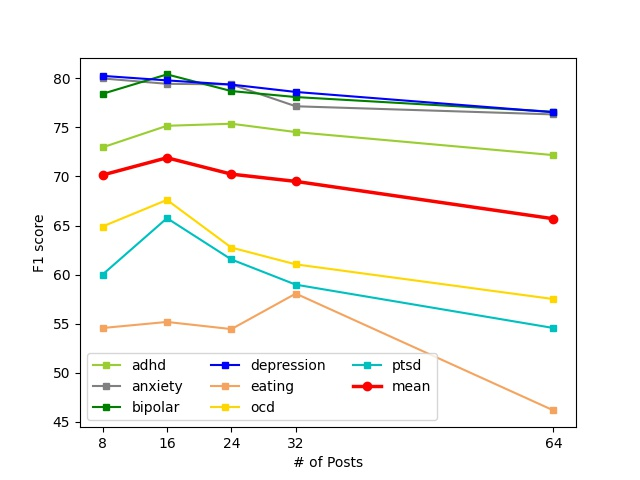
\includegraphics[width=\linewidth]{figures/post_num_impact.jpg}
    \caption{Impact of the number of selected posts on each disease and the mean F1.}
    \label{fig:post_num}
\end{figure}

\begin{figure*}[t]
    \centering
    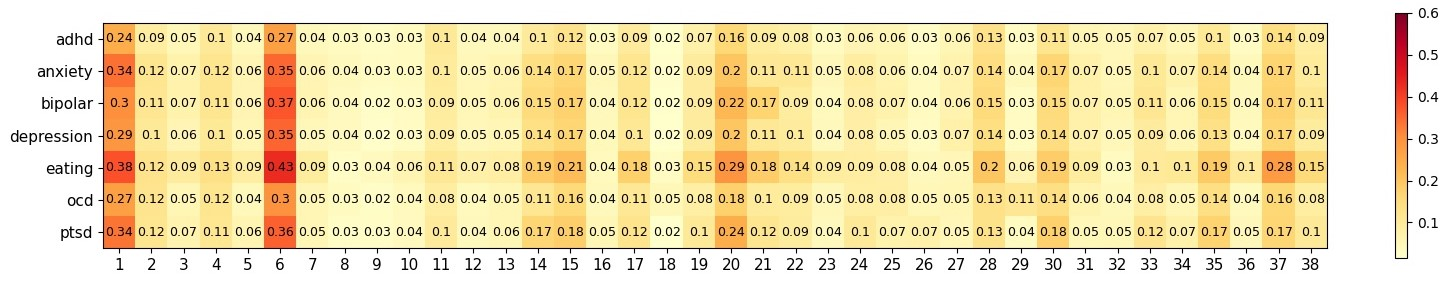
\includegraphics[width=0.9\linewidth]{figures/symp_contribution_wo_attn_wo_dsm.jpg}
    \caption{Symptom contribution for MDD without the selection by attention score.}
    \label{fig:symp_contribution_wo_attn}
\end{figure*}

\begin{table*}[t]
    \centering
    \resizebox{\textwidth}{15mm}{
    \begin{tabular}{m{1.5cm}|m{0.08cm}m{0.08cm}m{0.08cm}m{0.08cm}m{0.08cm}m{0.08cm}m{0.08cm}m{0.08cm}m{0.08cm}m{0.08cm}m{0.08cm}m{0.08cm}m{0.08cm}m{0.08cm}m{0.08cm}m{0.08cm}m{0.08cm}m{0.08cm}m{0.08cm}m{0.08cm}m{0.08cm}m{0.08cm}m{0.08cm}m{0.08cm}m{0.08cm}m{0.08cm}m{0.08cm}m{0.08cm}m{0.08cm}m{0.08cm}m{0.08cm}m{0.08cm}m{0.08cm}m{0.08cm}m{0.08cm}m{0.08cm}m{0.08cm}m{0.08cm}}
    \hline
    Disease          & 1 & 2 & 3 & 4 & 5 & 6 & 7 & 8 & 9 & 10 & 11 & 12 & 13 & 14 & 15 & 16 & 17 & 18 & 19 & 20 & 21 & 22 & 23 & 24 & 25 & 26 & 27 & 28 & 29 & 30 & 31 & 32 & 33 & 34 & 35 & 36 & 37 & 38 \\
    \hline
    ADHD & & & & & & & & &\checkmark &\checkmark &\checkmark & & & & & & & & & & & & & & & & &\checkmark & & & & & & & & & & \\
    \hline
    Anxiety &\checkmark &\checkmark &\checkmark & &\checkmark &\checkmark &\checkmark &\checkmark &\checkmark & &\checkmark & &\checkmark & & & & & & & & &\checkmark & &\checkmark & & & & & &\checkmark & &\checkmark &\checkmark &\checkmark &\checkmark &\checkmark & &\checkmark \\
    \hline
    Bipolar & & & & &\checkmark &\checkmark & & &\checkmark & &\checkmark & & &\checkmark &\checkmark & & & & &\checkmark &\checkmark & & & &\checkmark & &\checkmark &\checkmark & & & & &\checkmark & & & &\checkmark &\checkmark \\
    \hline
    Depression & & & & &\checkmark &\checkmark & &\checkmark &\checkmark & &\checkmark &\checkmark & &\checkmark &\checkmark & & & & & & & & & & & &\checkmark & & & &\checkmark &\checkmark &\checkmark & & & &\checkmark &\checkmark \\
    \hline
    Eating & & & & & &\checkmark & &\checkmark & & & & & & &\checkmark & &\checkmark & &\checkmark & & & &\checkmark &\checkmark & & &\checkmark & &\checkmark & & & &\checkmark & & & &\checkmark &\checkmark \\
    \hline
    OCD &\checkmark & & & & &\checkmark & & & & & & & & & & & &\checkmark & & & & & & & & & & &\checkmark & & & & & & & & & \\
    \hline
    PTSD &\checkmark &\checkmark & &\checkmark & & & & & & &\checkmark & & & &\checkmark &\checkmark & & &\checkmark &\checkmark & & & & & &\checkmark &\checkmark & & & &\checkmark &\checkmark &\checkmark & & & & &\checkmark \\
    \hline
    \end{tabular}}
    \caption{Symptoms of 7 mental disorders summarized from DSM-5.}
    \label{tab:symp_of_dsm5}
\end{table*}

\section{Detailed Symptom Contribution Results}
\label{apd:symp_contribution}
We use serial numbers to represent symptoms in Figure \ref{fig:symp_contribution}, and provide the corresponding symptom names in Table \ref{tab:symp_id} for reference. 
\begin{table}[ht]
    \small
    \centering
    \begin{tabular}{m{0.4cm}m{6cm}}
    \hline
    id & Symptom  \\
    \hline
    1&Anxious Mood 	\\
    2&Autonomic symptoms	\\
    3&Cardiovascular symptoms		\\
    4&Catatonic behavior\\
    5&Decreased energy tiredness fatigue	\\
    6&Depressed Mood\\
    7&Gastrointestinal symptoms	\\
    8&Genitourinary symptoms	\\
    9&Hyperactivity agitation	\\
    10&Impulsivity		\\
    11&Inattention	\\
    12&Indecisiveness	\\
    13&Respiratory symptoms\\
    14&Suicidal ideas	\\
    15&Worthlessness and guilty	\\
    16&Avoidance of stimuli	\\
    17&Compensatory behaviors to prevent weight gain	\\
    18&Compulsions		\\
    19&Diminished emotional expression		\\
    20&Do things easily get painful consequences	\\
    21&Drastic shift in mood and energy	\\
    22&Fear about social situations	\\
    23&Fear of gaining weight	\\
    24&Fears of being negatively evaluated	\\
    25&Flight of ideas	\\
    26&Intrusion symptoms	\\
    27&Loss of interest or motivation	\\
    28&More talkative\\
    29&Obsession	\\
    30&Panic fear	\\
    31&Pessimism	\\
    32&Poor memory	\\
    33&Sleep disturbance	\\
    34&Somatic muscle		\\
    35&Somatic symptoms others		\\
    36&Somatic symptoms sensory	\\
    37&Weight and appetite change	\\
    38&Anger Irritability	\\
    \hline
    \end{tabular}
    \caption{Id and its corresponding symptoms}
    \label{tab:symp_id}
\end{table}

We also provide another heatmap calculated without the assistance of attention scores (see Figure \ref{fig:symp_contribution_wo_attn}) for comparison.
For each disease, we calculate the symptom contribution among its diagnosed users similar to Figure \ref{fig:symp_contribution}. For each user with disease $d$, we simply add the averaged symptom probability vector of all the 16 posts to the disease-specific symptom contribution vector, without selecting the post with highest attention score.
Finally, we normalized the symptom contribution vectors by dividing the number of users with each disease, and we can obtain the symptom contribution heat map (Figure \ref{fig:symp_contribution_wo_attn}). 

Figures \ref{fig:symp_contribution} and \ref{fig:symp_contribution_wo_attn} respectively illustrate the heatmap with and without attention scores, indicating the differences in symptom contribution between diseases becomes more significant with the help of attention scores, further proving that the psychiatric "experts" can make it easier for the MDD model to distinguish between various mental diseases. 
%Comparing the heatmap with () and without (Figure \ref{fig:symp_contribution_wo_attn}) attention scores, we can find out that the 
% What's more, the attention-assisted symptom contribution are more consistent with DSM-5. For example, in figure \ref{fig:symp_contribution_wo_attn}, "Inattention" does not contribute much to ADHD; "depressed mood" contributes more to eating disorder rather than depression.

%To compare the discoveries from PsyEx and well-recognized clinical knowledge, we show the symptoms of 7 mental disorders in Table \ref{tab:symp_of_dsm5}, summarized in the knowledge graph from \citet{Zhang2022SymptomIF} mainly based on DSM-5. 
For comparison, we demonstrate the symptom-disease connection extracted from the diagnosis criteria DSM-5 in Table \ref{tab:symp_of_dsm5}. 
We can see much agreement between the findings drawn from our PsyEx model and the authoritative DSM-5, simultaneously with some inconsistencies, possibly due to the following reasons. First, there are many users with multiple diseases (Table \ref{tab:dis_num_distribution}), that our model learned to pay more attention to the common symptoms shared among these diseases.
Further, as a diagnostic criteria, DSM-5 tend to focus on the distinctive symptoms of each disease (e.g. "intrusion thoughts" for PTSD, "compulsion" for OCD) rather than the common ones (e.g. depression mood, anxious mood). However, these common symptoms can be generally meaningful to distinguish patients of most disorders from control users, so they are highly weighted by our PsyEx model.
